\documentclass[12pt]{article}
\usepackage{setspace,graphicx,amsmath,geometry,fontspec,titlesec,soul,bm,subfigure}
\titleformat{\section}[block]{\LARGE\bfseries}{\arabic{section}}{1em}{}[]
\titleformat{\subsection}[block]{\Large\bfseries\mdseries}{\arabic{section}.\arabic{subsection}}{1em}{}[]
\titleformat{\subsubsection}[block]{\normalsize\bfseries}{\arabic{subsection}-\alph{subsubsection}}{1em}{}[]
\titleformat{\paragraph}[block]{\small\bfseries}{[\arabic{paragraph}]}{1em}{}[]
\setmainfont{Times New Roman}
\renewcommand{\baselinestretch}{1.15}
\renewcommand\contentsname{Inhaltverzeichnis}
\geometry{a4paper,left=2.5cm,right=2.5cm,top=2.5cm,bottom=2.5cm}
\begin{document}
	\newpagestyle{main}{            
		\sethead{Ziqing Yu \& Roman Germann}{Orthophotogenerierung}{3218051 \& 322520}     
		\setfoot{}{\thepage}{}     
		\headrule                                     
		\footrule                                       
	}
	\pagestyle{main}
\tableofcontents
\newpage
\section{Theoretischer Teil}
Unter Resampling versteht man verschiedene Verfahren, mit denen die Grauwertmatrix bei einer geometrischen Transformation digitaler Bilder abgeleitet werden kann. Beim Resampling geht es um die Interpolation der diskreten Grauwerte der Matrix des transformierten Bildes zwischen benachbarten Pixeln des Ausgangsbildes. Die Bildelemente der neu entstehenden Matrix überdecken sich, wie des Eingabebildes, nicht vollständig. Da sich die neuen Bildelemente aus Teilbildelementen der Eingabebildmatrix zusammensetzen, muss festgelegt werden, wie die Grauwertzuweisung erfolgen soll. \newline
\newline
Es gibt folgende Verfahren:
\begin{itemize}
\item Nearest-Neighbour: Der nächstgelegene Grauwert im Eingabebild wird übernommen 
\item bilineare Interpolation: zwischen den vier benachbarten Grauwerten im Eingabenbild wird in Zeilen- und Spaltenrichtung linear interpoliert 
\item kubische Konvolution : zwischen den vier mal vier umliegenden Grauwerten im Eingabebild wird mit Gleichungen dritten Grades interpoliert 
\end{itemize}
Die Verfahren unterscheiden sich also im Wesentlichen in der Anzahl der verwendeten Grauwerte sowie der Art der Interpolation(linear/kubisch). Häufig wird die bilineare Interpolation verwendet, da diese einen guten Kompromiss zwischen Genauigkeit und Rechengeschwindigkeit bietet. Eine ideale Abtastfunktion ist die sinc-Funktion. \newline
\newline
Objektpunkt liegt $10\ m$ über Oberfläche, also $\Delta Z = 10\ m$,  Kamerakonstant ist $c = 120\ mm$ also $0,12\ m$,  in Bild gibt es $7680 \times 13824$ Pixel, Pixelgröße ist $12 \mu m$, dann ist $\Delta r' = 12 \mu m \cdot 7680 = 0.0922\ m$ in Flugrichtung und $12 \mu m \cdot 13824 = 0.1659 \mu m $ quer zur Flugrichtung. 
\begin{gather*}
\Delta r' = \Delta R \cdot \frac{c}{h_g} = \Delta Z \cdot \frac{r'}{h_g} = \Delta Z \frac{r'}{m \cdot c} \\
m = \frac{GSD}{\Delta Pixel}
\end{gather*}
\begin{table}[ht] \centering 
	\begin{tabular}{|l|l|l|l|}
		\hline
		GSD                   & 5cm     & 10cm    & 20cm    \\ \hline
		In Flugrichtung       & 1.843mm & 0.922mm & 0.461mm \\ \hline
		Quer zur Flugrichtung & 3.318mm & 1.659mm & 0.829mm \\ \hline
	\end{tabular}
\end{table}
\newline
Die Überdeckung soll groß sein, damit für einen Bereich mehrere Bild existieren und Radialversatz wird geringer sein. \newline
\newline
Aufnahmekonfiguration: die Überdeckung soll möglichst groß sein. Wenn Kamerakonstante $c$ größer, also Öffnungswinkel kleiner ist, ist Radialversatz kleiner. 
\section{Praktischer Teil}
\subsection{Visualisierung und Generierung einer 3D-Perspektivansicht}
Mit DTMMater kann man die Visualisierung realisieren.
\begin{figure*}[ht]\centering
	\subfigure[DGM]{
		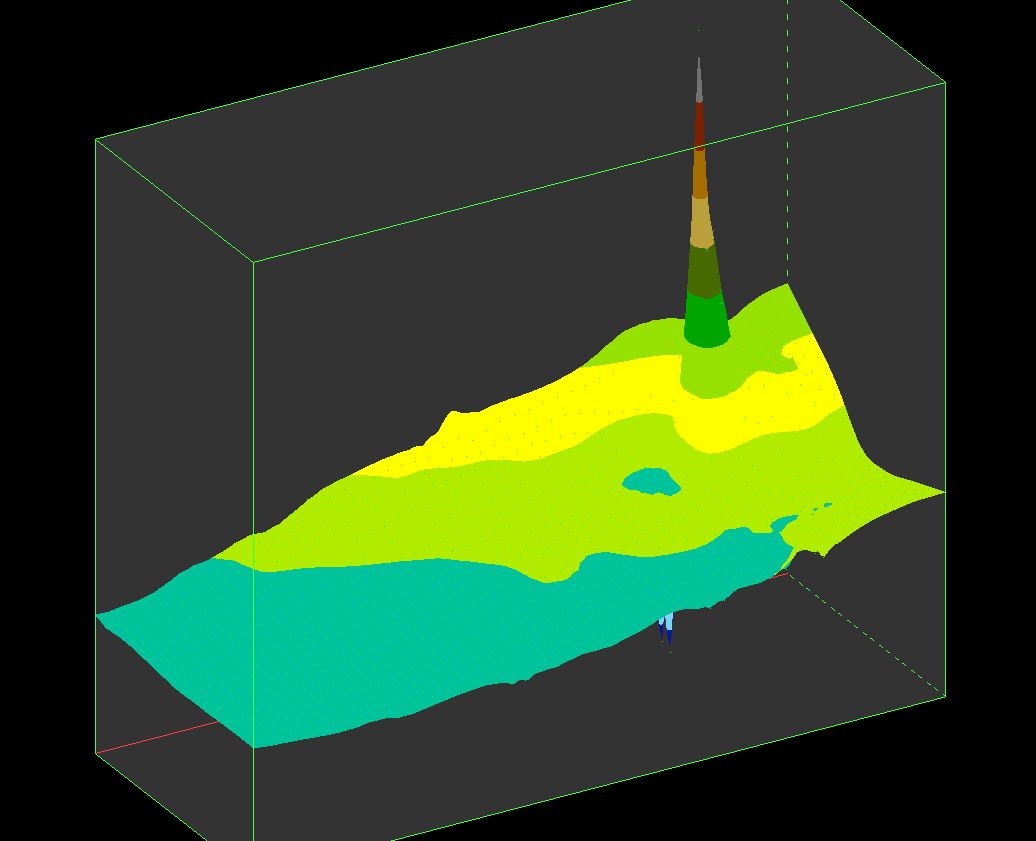
\includegraphics[width=0.45\textwidth]{DGM.png}}
	\subfigure[DOM]{
		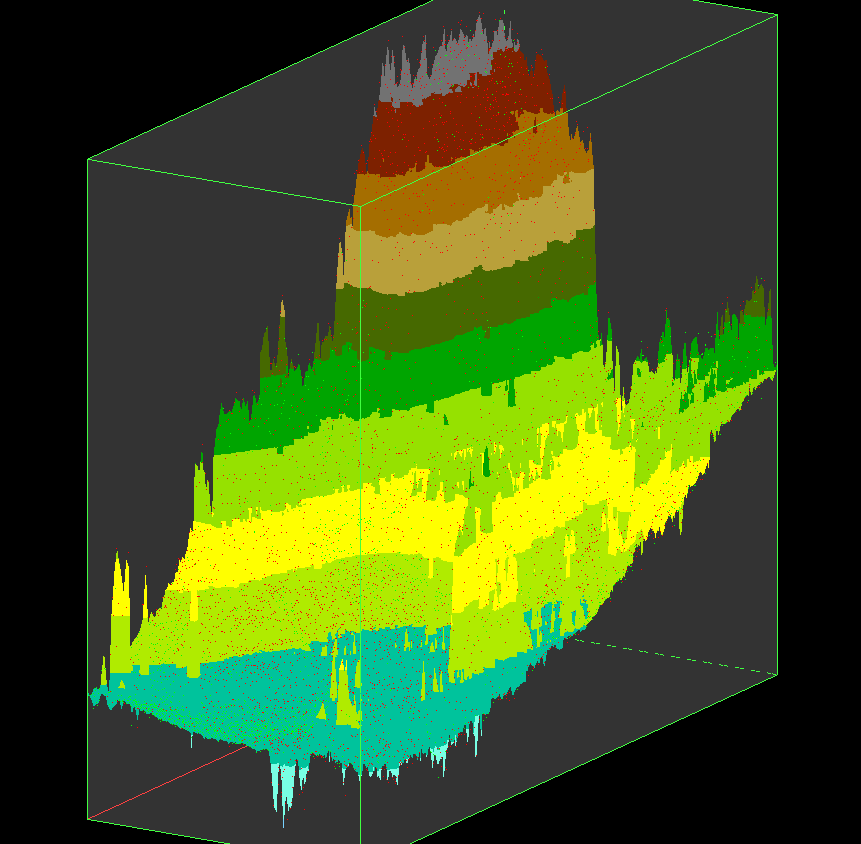
\includegraphics[width=0.45\textwidth]{DOM.png}}
\end{figure*}
\newline
Aus dem Graph ist es deutlich zu sehen, dass DOM flacher als DGM ist, weil Orthophoto bei DOM digitale Oberfläche zeigt und das Bild mit DGM die Geländefläche darstellt. Die Auflösung mit DOM ist auch höher.
\newpage
\subsection{Orthophotogenerieung}
\subsubsection{minimale Pixelgröße}
$0.02 \ m$ ist die minimale Pixelgröße. GSD bedeutet groud sample distance, also Bodenauflösung. Unter Auflösung gibt es Geometrische Auflösung, Radiometrische Auflösung usw.
\subsubsection{DGM und DOM}
\begin{figure*}[ht]\centering
	\subfigure[DGM]{
		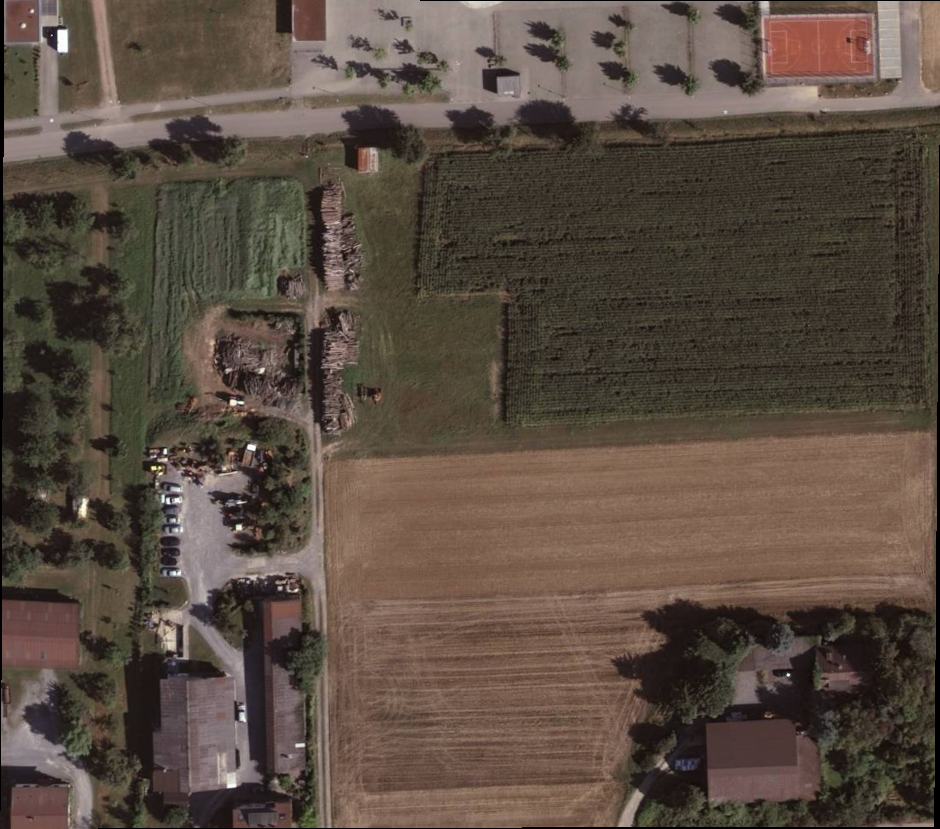
\includegraphics[width=0.55\textwidth]{FallDGM.png}}
	\subfigure[DOM]{
		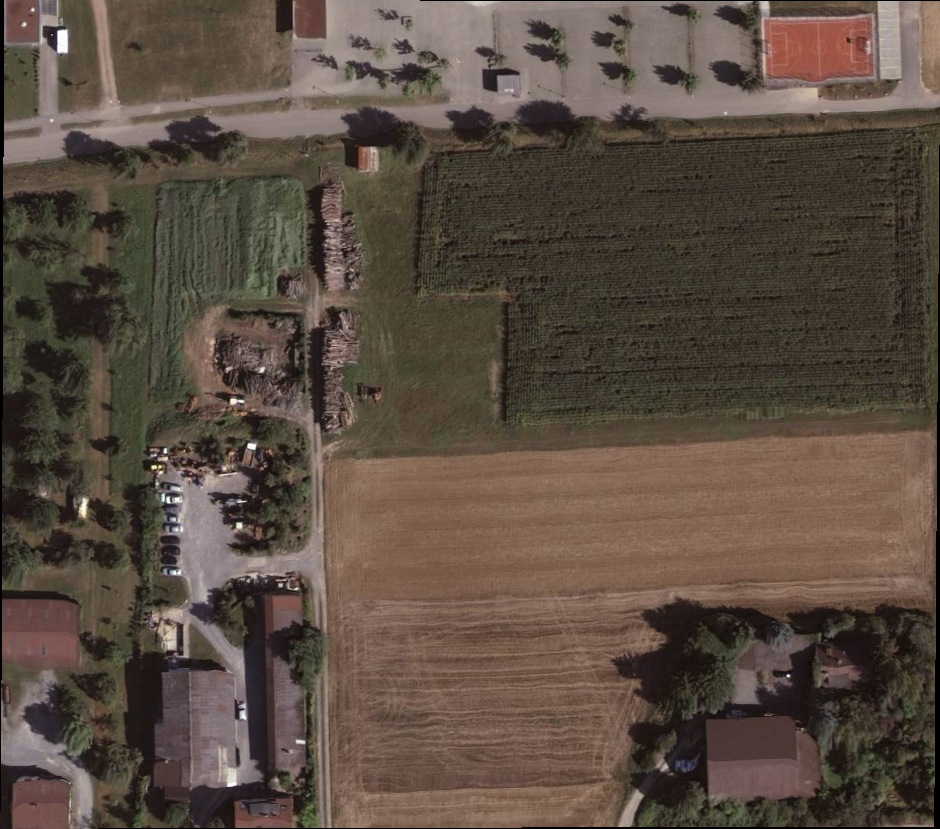
\includegraphics[width=0.55\textwidth]{FallDOM.png}}
\end{figure*}
\noindent Im Orthophoto mit DOM ist Höhenversatzfehler deutlich größer, aber die Koordinaten sind ähnlich. \newpage
\subsubsection{Fall 0}
DGM, strenges Verfahren, bilineare Interpolation Auflösung:0.2m \newline
\begin{figure*}[ht]\centering
	\subfigure[DGM]{
		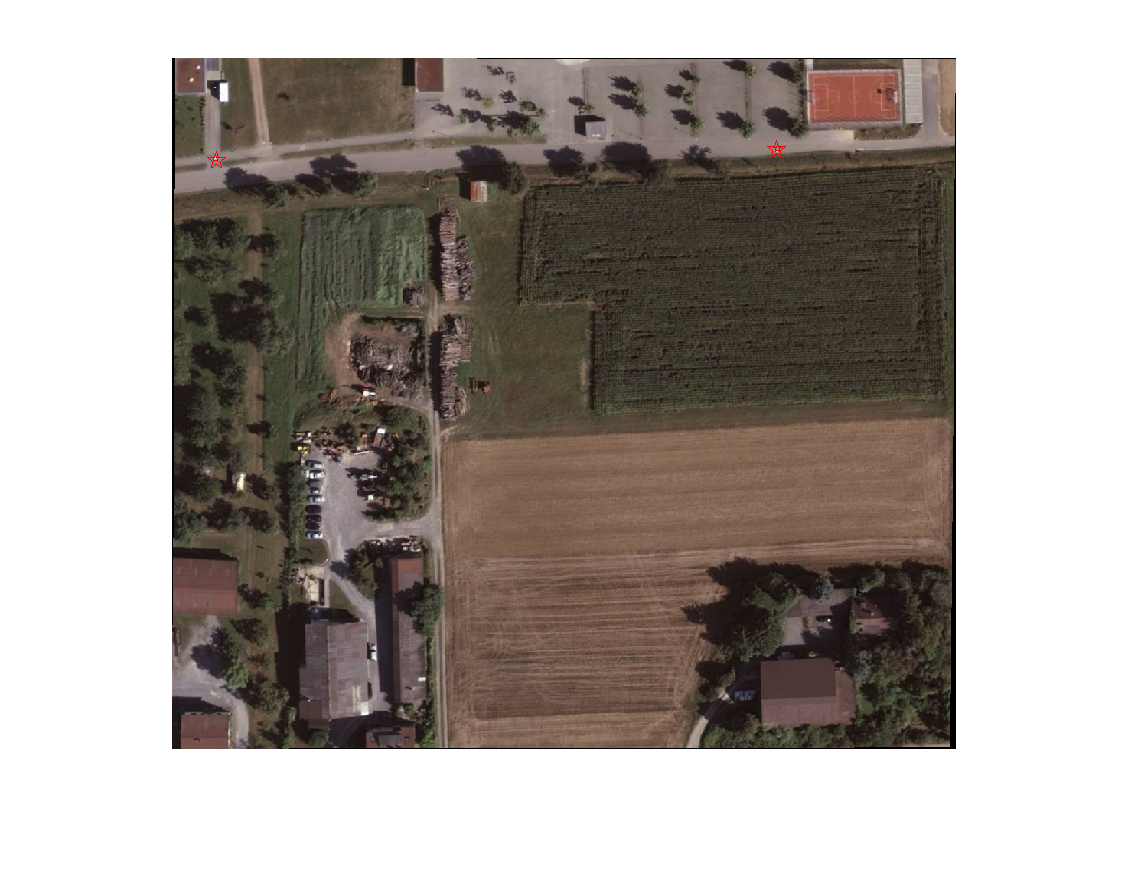
\includegraphics[width=0.9\textwidth]{Fall0.png}}
\end{figure*}
\newline
Markierte Punkte sind die Festpunkten 9002(link) und 9001(recht), deren Koordinaten darunter liegen.
\begin{table}[ht] \centering
	\begin{tabular}{|l|l|l|}
		\hline
		Punkt & E          & N           \\ \hline
		9002  & 497255.426 & 5421572.643 \\ \hline
		9001  & 4974232768 & 5421574.723 \\ \hline
	\end{tabular}
\end{table}
\newpage
\subsubsection{Fall A}
DGM, strenges Verfahren, bilineare Interpolation, Bodenpixelgröße = 1m, 0.5m, 0.2m 
\begin{figure*}[ht]\centering
	\subfigure[1m]{
		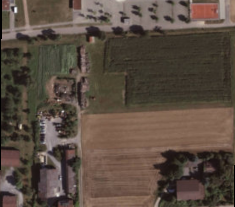
\includegraphics[width=0.45\textwidth]{FallA1m.png}}
	\subfigure[0.5m]{
		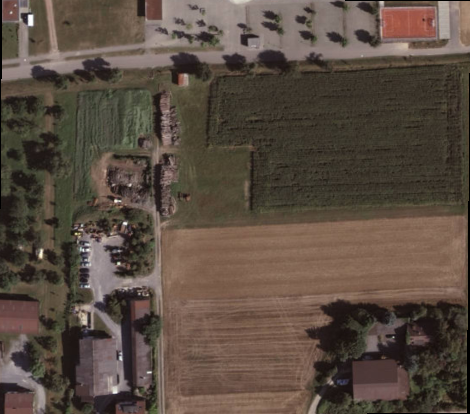
\includegraphics[width=0.45\textwidth]{FallA50cm.png}}
	\subfigure[0.2m]{
		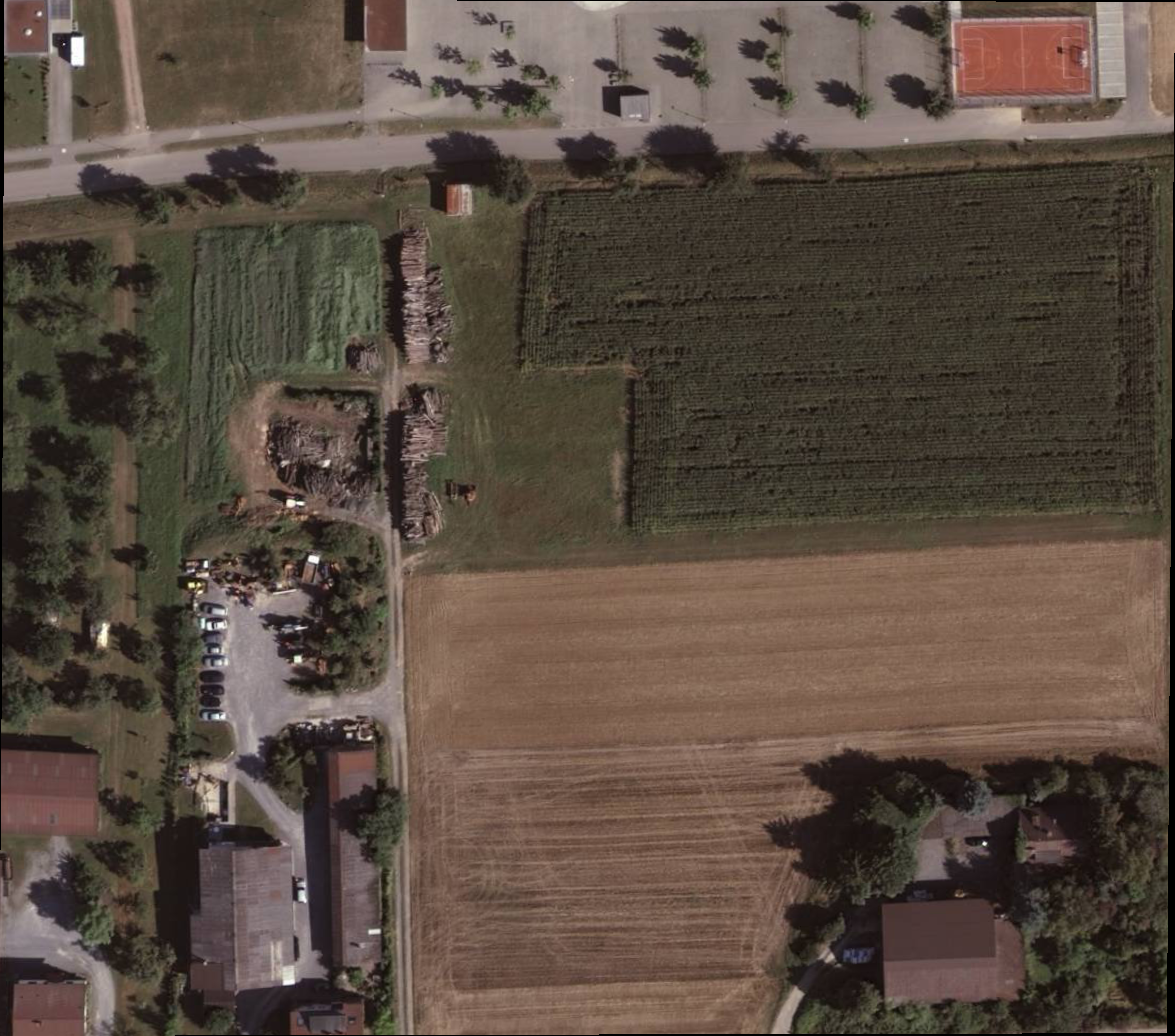
\includegraphics[width=0.45\textwidth]{FallA20cm.png}}
\end{figure*}
\newline
Bei verschiedene Bodenpixelgröße ändert sich nur die Schärfe.
\newpage
\subsubsection{Fall B}
DGM, strenges Verfahren, Bodenpixelgröße = 0.25m 
\begin{figure*}[ht]\centering
	\subfigure[bilineare Interpolation]{
		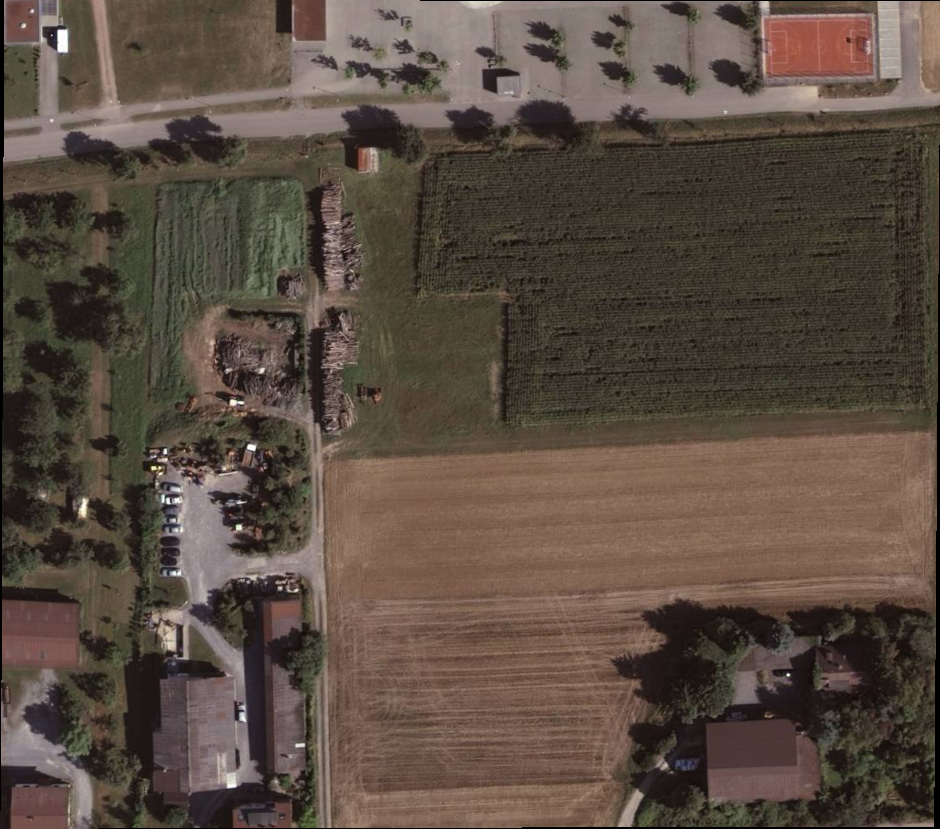
\includegraphics[width=0.45\textwidth]{FallBbilinear.png}}
	\subfigure[Nearest-Neighbour]{
		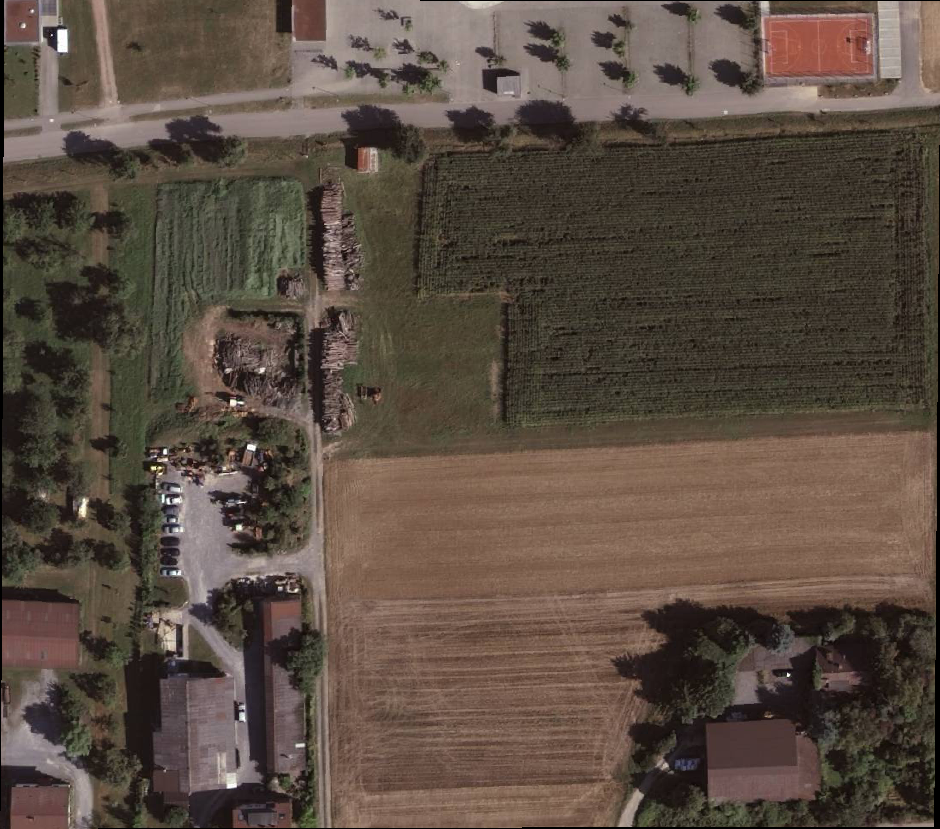
\includegraphics[width=0.45\textwidth]{FallBneighbour.png}}
	\subfigure[kubische Konvolution]{
		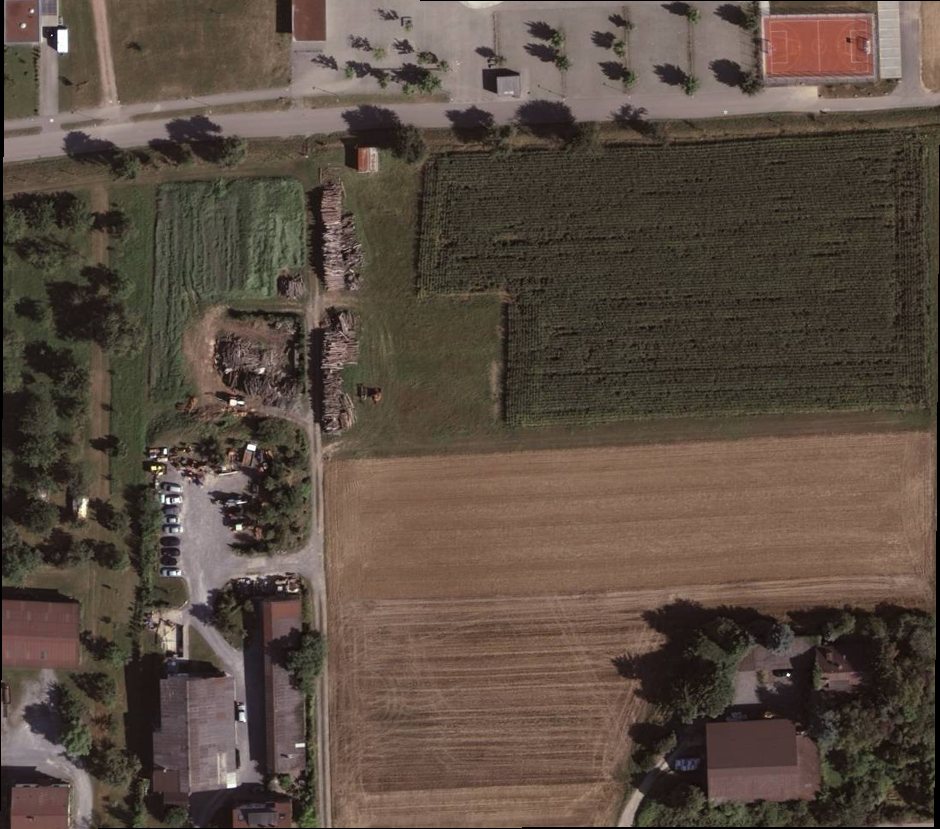
\includegraphics[width=0.45\textwidth]{FallBcubic.png}}
\end{figure*}
\newline
Es gibt fast keine Unterschied auf Bildern mit verschiedenen Interpolationsverfahren. 
\newpage
\subsubsection{Fall C}
DGM, Bodenpixelgröße = 0.25m, bilineare Interpolation
\begin{figure*}[ht]\centering
	\subfigure[Strenger Ansatz]{
		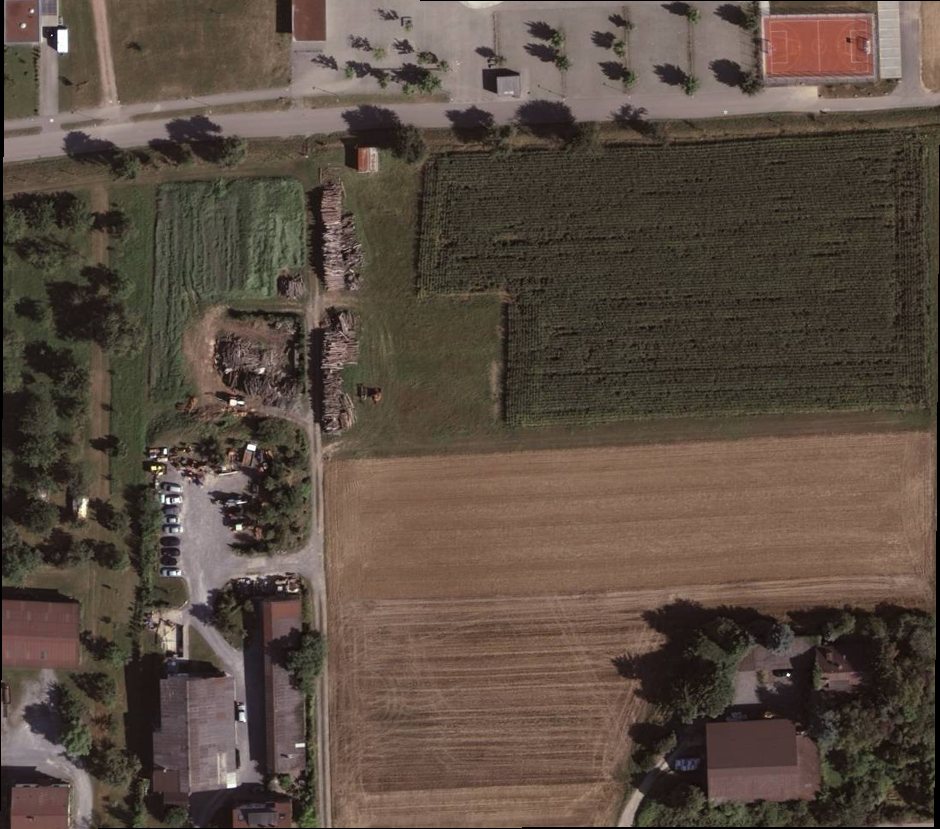
\includegraphics[width=0.45\textwidth]{FallCstreng.png}}
	\subfigure[Ankerpunkte 10 m]{
		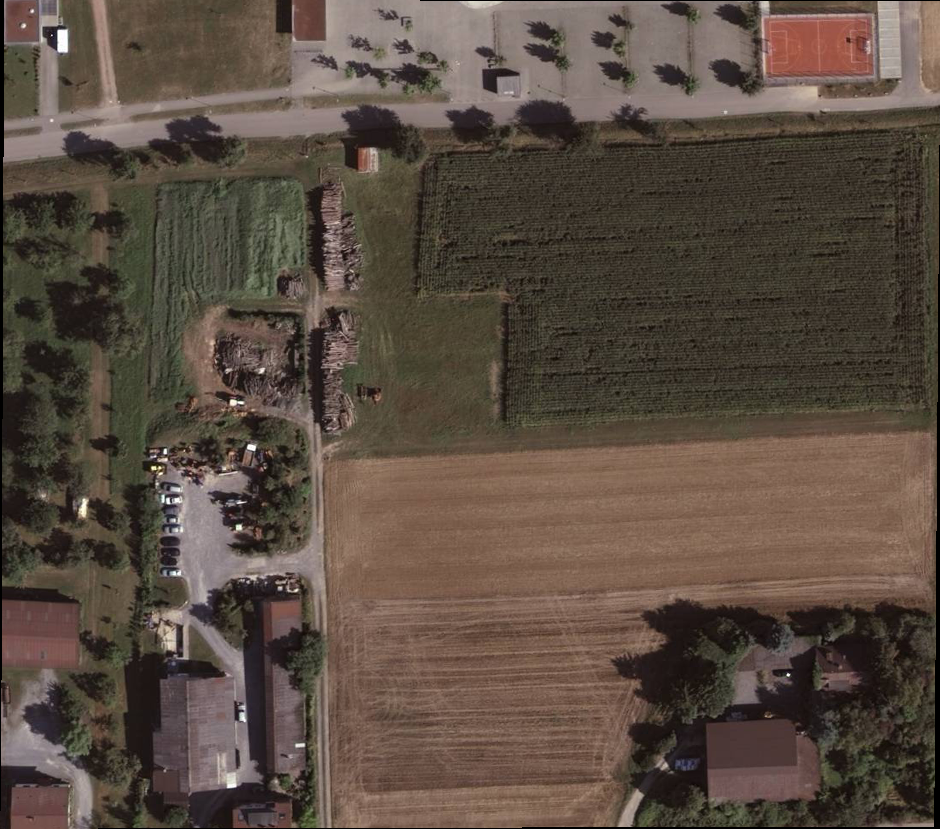
\includegraphics[width=0.45\textwidth]{FallC025.png}}
	\subfigure[Ankerpunkte 50 m]{
		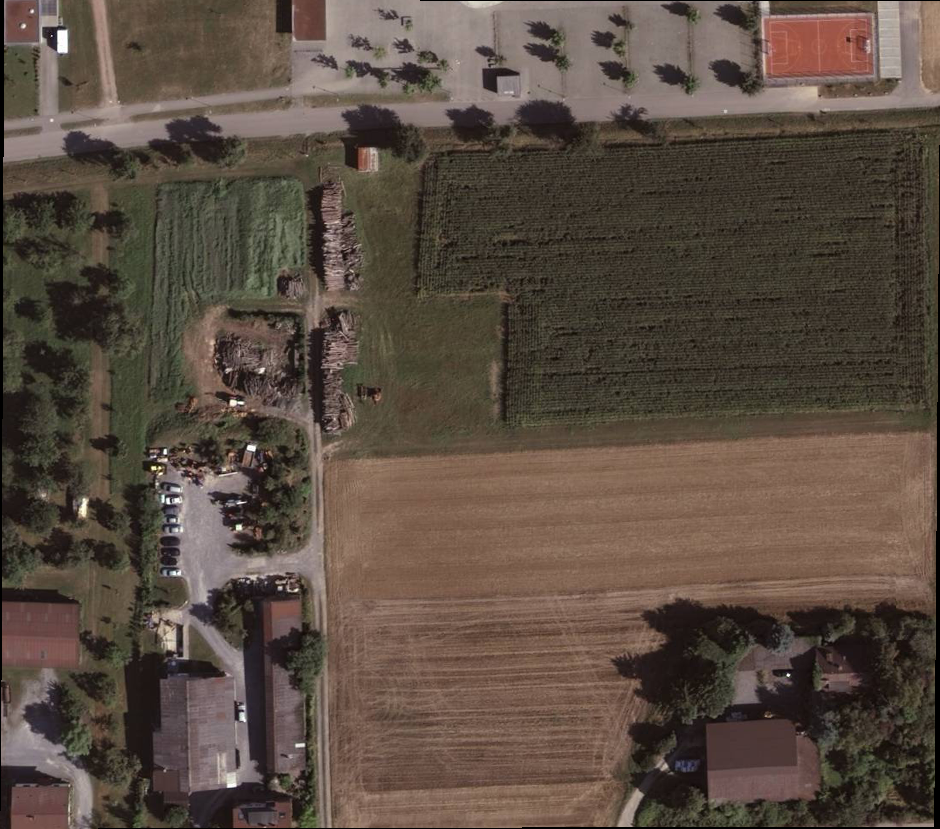
\includegraphics[width=0.45\textwidth]{FallC50.png}}
\end{figure*}
\newline
Punktekoordinaten von Strenger Ansatz, Ankerpunkte Maschenweite gleich 10m und Ankerpunkte Maschenweite gleich 50m. In Vergleich mit den Koordinaten bei Fall0 ist die Änderung sehr wenig. 
\begin{table}[ht] \centering
	\begin{tabular}{|l|l|l|}
		\hline
		Punkt & E          & N           \\ \hline
		9002  & 497255.488 & 5421572.924 \\ \hline
		9001  & 497423.652 & 5421575.226 \\ \hline
	\end{tabular}
\begin{tabular}{|l|l|l|}
	\hline
	Punkt & E          & N           \\ \hline
	9002  & 497255.253 & 5421572.771 \\ \hline
	9001  & 497423.728 & 5421575.811 \\ \hline
\end{tabular}
\begin{tabular}{|l|l|l|}
	\hline
	Punkt & E          & N           \\ \hline
	9002  & 497255.666 & 5421572.803 \\ \hline
	9001  & 497423.768 & 5421574.963 \\ \hline
\end{tabular}
\end{table}
\newpage
\subsubsection{Fall D}
DGM, Bodenpixelgröße = 0.25m, bilineare Interpolation, strenger Ansatz. Mittelere Höhe ist 335 Meter.
\begin{figure*}[ht]\centering
	\subfigure[mittelere Höhe]{
		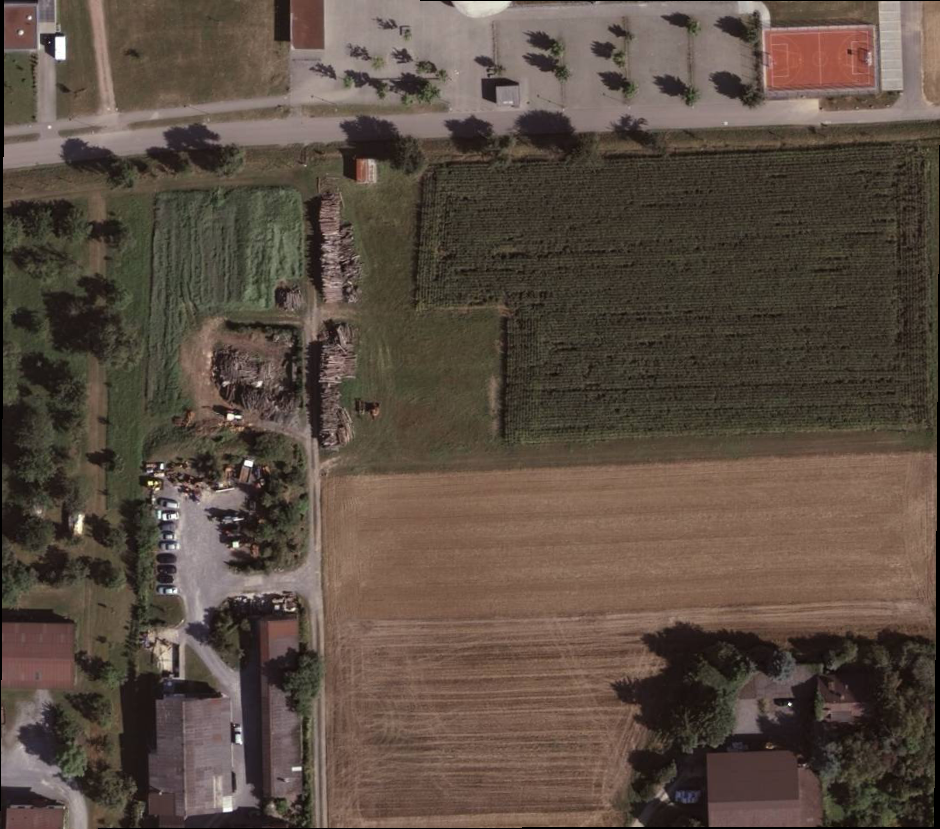
\includegraphics[width=0.45\textwidth]{FallDmittel.png}}
	\subfigure[50 meter höher]{
		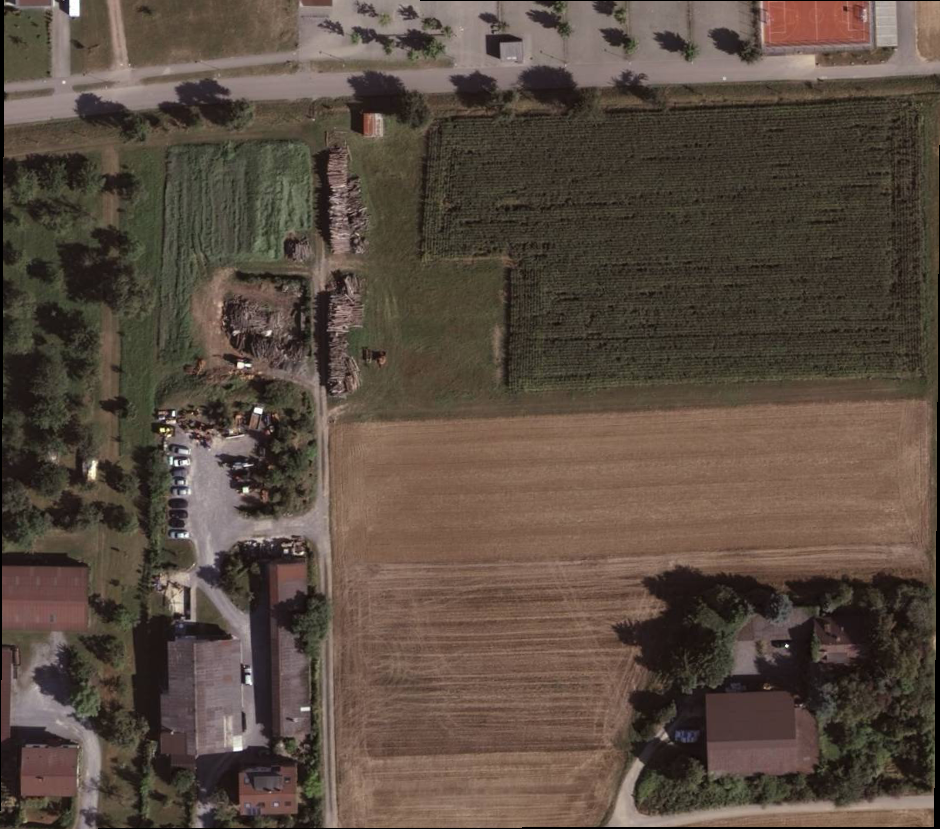
\includegraphics[width=0.45\textwidth]{FallD50+.png}}
	\subfigure[50 meter niedriger]{
		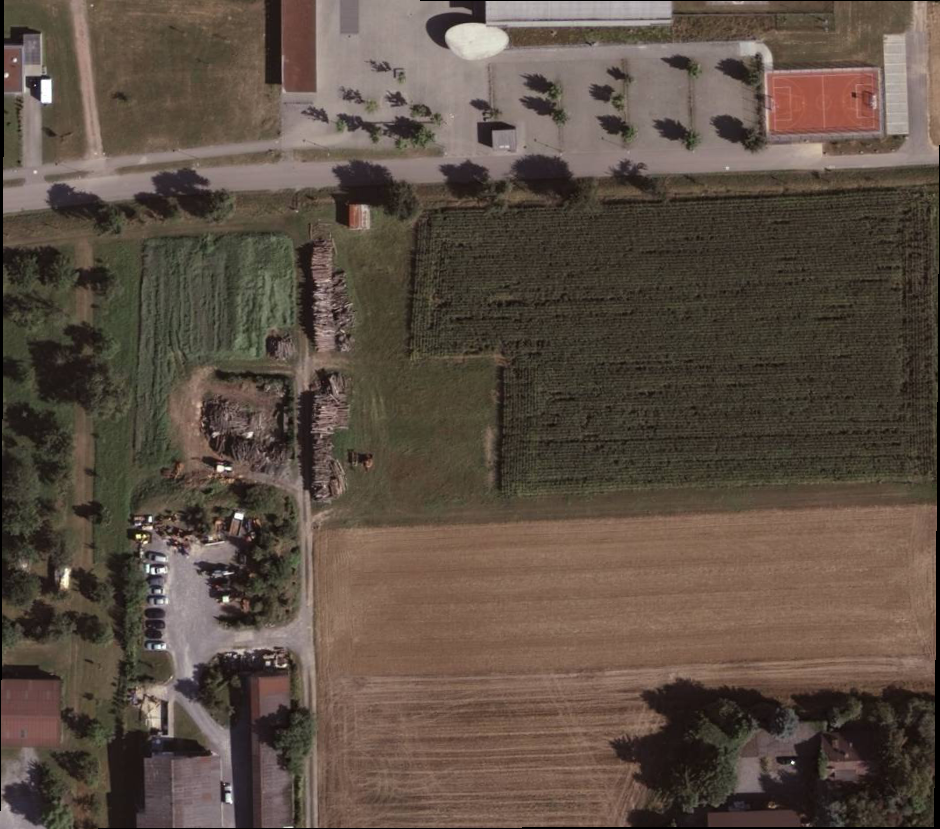
\includegraphics[width=0.45\textwidth]{FallD50-.png}}
\end{figure*}
\newline
Tabelle sind die Festpunkte Koordinaten wenn: 
\begin{itemize}
\item Geländeebene in Höhe der mittleren Geländehöhe.
\item Geländeebene 50m über mittlerer Geländehöhe.
\item Geländeebene 50m unter mittlerer Geländehöhe
\end{itemize}
\begin{table}[ht] \centering
	\begin{tabular}{|l|l|l|}
		\hline
		Punkt & E          & N           \\ \hline
		9002  & 497254.706 & 5421571.084 \\ \hline
		9001  & 497423.788 & 5421572.104 \\ \hline
	\end{tabular}
	\begin{tabular}{|l|l|l|}
	\hline
	Punkt & E          & N           \\ \hline
	9002  & 497258.345 & 5421582.440 \\ \hline
	9001  & 497423.448 & 5421583.320 \\ \hline
	\end{tabular}
	\begin{tabular}{|l|l|l|}
	\hline
	Punkt & E          & N           \\ \hline
	9002  & 497251.267 & 5421559.848 \\ \hline
	9001  & 497424.088 & 5421560.727 \\ \hline
	\end{tabular}
\end{table}
Es ist aus den Graphen zu sehen, dass der Bild sich verschoben hat mit verschieden Geländeebene Höhen. Die Koordinaten sind auch deutlich geändert mit verschiedenen Höhen. 
\end{document}
